\documentclass[conference]{IEEEtran}
\usepackage[utf8]{inputenc}
\usepackage[spanish]{babel}
\usepackage{amsmath,amssymb,amsfonts}
\usepackage{graphicx}
\usepackage{cite}
\usepackage{hyperref}
\usepackage{array}

\graphicspath{{../figures/}}

\newcommand{\vol}{\mathrm{vol}}
\newcommand{\cut}{\mathrm{cut}}
\newcommand{\Sobs}{S_{\mathrm{obs}}}
\newcommand{\Sfied}{S_{\mathrm{Fiedler}}}

\begin{document}

\title{Simetria, Degeneracion del Eigenspace de Fiedler y Coordinacion Axial en Seeking the Unicorn}

\author{\IEEEauthorblockN{Thomas Chisica}
\IEEEauthorblockA{Universidad del Rosario\\
Teoria de Grafos 2026-I\\
Profesor: Daniel Alfonso Bojaca Torres}}

\maketitle

\begin{abstract}
Este trabajo reanaliza el experimento \emph{Seeking the Unicorn} \cite{andrade2021} con una pregunta mas acotada que la del borrador inicial: cuando el tablero cuadrado $P_8 \boxtimes P_8$ tiene un eigenspace de Fiedler degenerado, \textit{las diadas humanas con divisiones espaciales claras se alinean con direcciones geometricamente privilegiadas?} Modelamos el tablero como un grafo de 64 nodos y 210 aristas, comparamos la particion humana observada contra el corte de Fiedler ingenuo y contra baselines axiales triviales, y complementamos la geometria con informacion mutua, divergencia de Jensen-Shannon y estabilidad inter-ventanas. En el tablero cuadrado se verifica $\lambda_2=\lambda_3\approx0.4164$, el corte de Fiedler ingenuo tiene conductancia $28/210=0.1333$ y los cortes axiales LR/TB tienen $22/210=0.1048$, usado aqui solo como baseline axis-aligned de referencia dentro de la familia comparada y no como optimo global de $h(G)$. Sobre 45 diadas auditadas, 29 entran al set primario de conductancia. Dentro de ese subconjunto, las diadas axiales muestran conductancia media $0.142$ frente a $0.714$ en las mixtas, junto con mayor $DLIndex$, mayor MI y mayor JSD. Sin embargo, la lectura debe ser critica: $\eta$ y $DLIndex$ se correlacionan fuertemente ($\rho=0.894$), y en este tablero el mejor baseline axis-aligned coincide numericamente con el baseline espectral sensible a simetria. Por tanto, el aporte actual es un reanalisis estructural parcial del fenomeno, util para las estrategias LR/TB pero insuficiente como explicacion total de SODCL. El siguiente paso natural es una manipulacion de ruptura de simetria del tablero.
\end{abstract}

\section{Introduccion}

La division espontanea del trabajo entre agentes sin comunicacion explicita es un problema central en ciencia cognitiva, sistemas multiagente y coordinacion colectiva \cite{andrade2021,goldstone2024}. En \emph{Seeking the Unicorn}, dos participantes buscan un objetivo oculto en una grilla de $8\times8$ y, con el tiempo, muchas diadas desarrollan convenciones espaciales que reducen redundancia y mejoran cobertura \cite{andrade2021}. Esa regularidad ya fue establecida por el trabajo original. El problema de este proyecto no es redescubrir que los humanos se coordinan, sino preguntar que agrega una lente de teoria espectral de grafos a la geometria del tablero.

El punto de partida es que el tablero con conectividad de rey se modela como el producto fuerte $P_8 \boxtimes P_8$ \cite{hammack2011}. En este grafo cuadrado, el segundo eigenvalor del Laplaciano combinatorial no es simple: el eigenspace de Fiedler es bidimensional. Eso implica que la biseccion espectral estandar no es unica y que distintas direcciones dentro del mismo subespacio pueden inducir cortes geometricamente muy distintos. La hipotesis acotada de este trabajo es la siguiente: \textbf{cuando las diadas humanas desarrollan divisiones espaciales nitidas, tienden a alinearse con direcciones axiales privilegiadas dentro del eigenspace degenerado.}

Este framing exige una lectura mas estricta que la del borrador anterior. No afirmamos que los humanos ``optimizan espectralmente'' en general, ni que el analisis actual explique todas las estrategias focales reportadas en SODCL. La evidencia de este repositorio es mas estrecha: cubre bien los casos izquierda-derecha y arriba-abajo, pero deja fuera estrategias como ``ALL/NOTHING'' o configuraciones no claramente bipartitas. El valor del proyecto depende entonces de si la lente espectral agrega interpretacion estructural y prediccion futura, no de si redescubre un resultado ya publicado.

\section{Datos, problema y alcance}

El experimento original contiene 60 rondas por diada \cite{andrade2021}, pero el dataset primario usado aqui es ``humans\_only\_absent.csv'', que conserva solo rondas con unicornio ausente. Por eso cada diada aporta menos observaciones que el total experimental, sin que esto constituya una inconsistencia del dataset.

El tablero se modela como el grafo
\[
G = P_8 \boxtimes P_8,
\]
con 64 nodos y 210 aristas. Cada celda es un vertice y dos celdas son adyacentes si estan a distancia de Chebyshev 1. Para una particion $(S,\bar S)$, la calidad geometrica se mide con conductancia:
\begin{equation}
h(S)=\frac{\cut(S,\bar S)}{\min(\vol(S),\vol(\bar S))}.
\end{equation}

La particion observada de una diada se extrae a partir de las frecuencias de visita tardias. Si $f_1(v)$ y $f_2(v)$ son las visitas acumuladas de los dos jugadores a la celda $v$ en rondas ``Round $\geq 40$'', definimos
\begin{equation}
\Sobs = \{v \in V : f_1(v) > f_2(v)\}.
\end{equation}
Esta discretizacion induce una biparticion dura que es util para conductancia, pero no agota toda la estructura conductual del experimento.

El set primario de analisis contiene solo diadas para las que esta particion dura es interpretable bajo una regla fija: dos jugadores presentes, rondas tardias disponibles, y tamano de $\Sobs$ entre 10 y 54 nodos. Esa regla deja 29 diadas en el analisis primario y excluye 16 casos extremos.

\begin{table}[t]
\caption{Flujo de muestra del analisis primario}
\label{tab:flow}
\centering
\begin{tabular}{|l|c|}
\hline
Etapa & Diadas \\
\hline
Auditadas en ``humans\_only\_absent.csv'' & 45 \\
Incluidas en el set primario & 29 \\
Excluidas por particion muy pequena & 8 \\
Excluidas por particion muy grande & 8 \\
\hline
\end{tabular}
\end{table}

Esta exclusion no es ruido tecnico arbitrario. Entre las 16 diadas excluidas, los modos de categoria tardia son ``ALL'' (7 casos), ``RS'' (6 casos) y ``NOTHING'' (3 casos). Eso delimita el alcance real del trabajo: la metrica de conductancia favorece escenarios de biparticion espacial razonable y no debe venderse como explicacion total del fenomeno SODCL.

\section{Metodologia}

\subsection{Baseline espectral y baselines no espectrales}

Sea $L=D-A$ el Laplaciano combinatorial del grafo. Computacionalmente se obtiene
\[
\lambda_2=\lambda_3\approx 0.4164,
\]
lo que confirma la degeneracion del eigenspace de Fiedler en el caso cuadrado. El corte de Fiedler ingenuo se define tomando el signo de un eigenvector numerico asociado a $\lambda_2$ \cite{fiedler1973,vonluxburg2007}. En paralelo, evaluamos tres baselines no espectrales triviales:
\begin{itemize}
\item particion izquierda-derecha (LR),
\item particion arriba-abajo (TB),
\item \emph{best axis-aligned}, que toma el mejor valor entre LR y TB.
\end{itemize}

Esta comparacion es obligatoria porque, en un tablero cuadrado, la interpretacion espectral puede quedar confundida con un simple sesgo cartesiano.

\subsection{Clasificacion axial vs mixed}

No usamos la variable externa \textit{Category} para definir el grupo principal. En cambio, la orientacion se obtiene del campo firmado de dominancia espacial, comparando su alineacion con plantillas LR y TB en tres ventanas temporales: 30--60, 40--60 y 50--60. Una diada se clasifica como:
\begin{itemize}
\item \textbf{LR} si domina de forma estable la orientacion horizontal,
\item \textbf{TB} si domina de forma estable la orientacion vertical,
\item \textbf{MIXED} en caso contrario.
\end{itemize}

Para el reporte principal agrupamos LR y TB bajo la etiqueta \textbf{axiales}. Las metricas temporales se toman de la orientacion estable entre ventanas.

\subsection{Metricas informacionales y de estabilidad}

Como complemento de la conductancia, medimos:
\begin{itemize}
\item \textbf{informacion mutua} $I(X;C)$ entre jugador y celda visitada \cite{cover2006},
\item \textbf{divergencia de Jensen-Shannon} entre las distribuciones de visita de ambos jugadores \cite{lin1991},
\item \textbf{especializacion suave} basada en el margen absoluto de dominancia,
\item \textbf{Jaccard inter-ventana} para cuantificar estabilidad de la particion.
\end{itemize}

La metrica comparativa principal es
\[
\eta = \frac{h(\Sfied)}{h(\Sobs)},
\]
donde valores mayores a 1 indican una particion humana mejor que el corte de Fiedler ingenuo, y valores menores a 1 indican lo contrario.

\section{Resultados}

\subsection{Invariantes del tablero}

Los baselines geometricos del tablero son estables y no dependen de las diadas:
\begin{itemize}
\item corte de Fiedler ingenuo: $h=28/210=0.1333$,
\item corte LR: $h=22/210=0.1048$,
\item corte TB: $h=22/210=0.1048$,
\item \emph{best axis-aligned}: $h=22/210=0.1048$.
\end{itemize}

El resultado importante aqui es ambiguo a proposito. Por un lado, la degeneracion del eigenspace explica por que el redondeo espectral ingenuo puede ser suboptimo. Por otro lado, en este tablero el mejor corte axial trivial coincide numericamente con el mejor corte ``espectral sensible a simetria''. Eso obliga a presentar el aporte como interpretacion estructural, no como victoria limpia sobre un baseline cartesiano.

\subsection{Separacion axial vs mixed en el set primario}

El set primario contiene 21 diadas axiales y 8 diadas mixtas. La Tabla~\ref{tab:primary} resume las metricas centrales. Las diferencias axial vs mixed son fuertes y consistentes: las diadas axiales tienen menor conductancia observada, mayor alineacion con el baseline ingenuo, mayor \textit{DLIndex}, y mayor especializacion informacional.

\begin{table}[t]
\caption{Resultados en el set primario}
\label{tab:primary}
\centering
\resizebox{\columnwidth}{!}{
\begin{tabular}{|l|c|c|c|c|c|c|}
\hline
Grupo & $n$ & $h(\Sobs)$ & $\eta$ & DLIndex & MI & JSD \\
\hline
Axiales & 21 & 0.142 & 1.120 & 0.919 & 0.839 & 0.842 \\
Mixed & 8 & 0.714 & 0.196 & 0.514 & 0.260 & 0.284 \\
\hline
\end{tabular}
}
\end{table}

Las pruebas de Mann-Whitney refuerzan esa separacion: $h(\Sobs)$ ($p=3.07\times10^{-5}$), $DLIndex$ ($p=1.33\times10^{-4}$), MI ($p=4.23\times10^{-4}$) y JSD ($p=3.50\times10^{-4}$). El contraste mas fuerte aparece en la geometria: las mixtas permanecen lejos de cualquier biparticion axial de baja conductancia.

La lectura por diadas tambien es instructiva. Entre las 21 diadas axiales:
\begin{itemize}
\item 14 alcanzan exactamente el valor axial de referencia $22/210$,
\item 3 mejoran el corte de Fiedler ingenuo sin alcanzar el minimo axial,
\item 4 no mejoran el corte ingenuo.
\end{itemize}
Entre las 8 diadas mixed, ninguna supera al corte de Fiedler ingenuo. Este patron es mas honesto que la frase fuerte del borrador previo: no todas las diadas focales convergen al minimo, pero muchas de las axiales si lo alcanzan o se acercan a el.

\subsection{Robustez temporal}

La separacion axial vs mixed no depende de una sola ventana. Al imponer orientacion estable entre 30--60, 40--60 y 50--60, las diadas axiales conservan mejor geometria, mayor especializacion y mas estabilidad inter-ventana:
\begin{itemize}
\item $h_{40-60}$: axial 0.119 vs mixed 0.701 ($p=8.07\times10^{-6}$),
\item especializacion suave: axial 0.906 vs mixed 0.492 ($p=1.99\times10^{-4}$),
\item Jaccard medio: axial 0.934 vs mixed 0.651 ($p=1.79\times10^{-3}$).
\end{itemize}

En otras palabras, las diadas axiales no solo producen mejores cortes; tambien sostienen esa organizacion con mayor claridad funcional a traves del tiempo.

\begin{figure}[t]
\centering
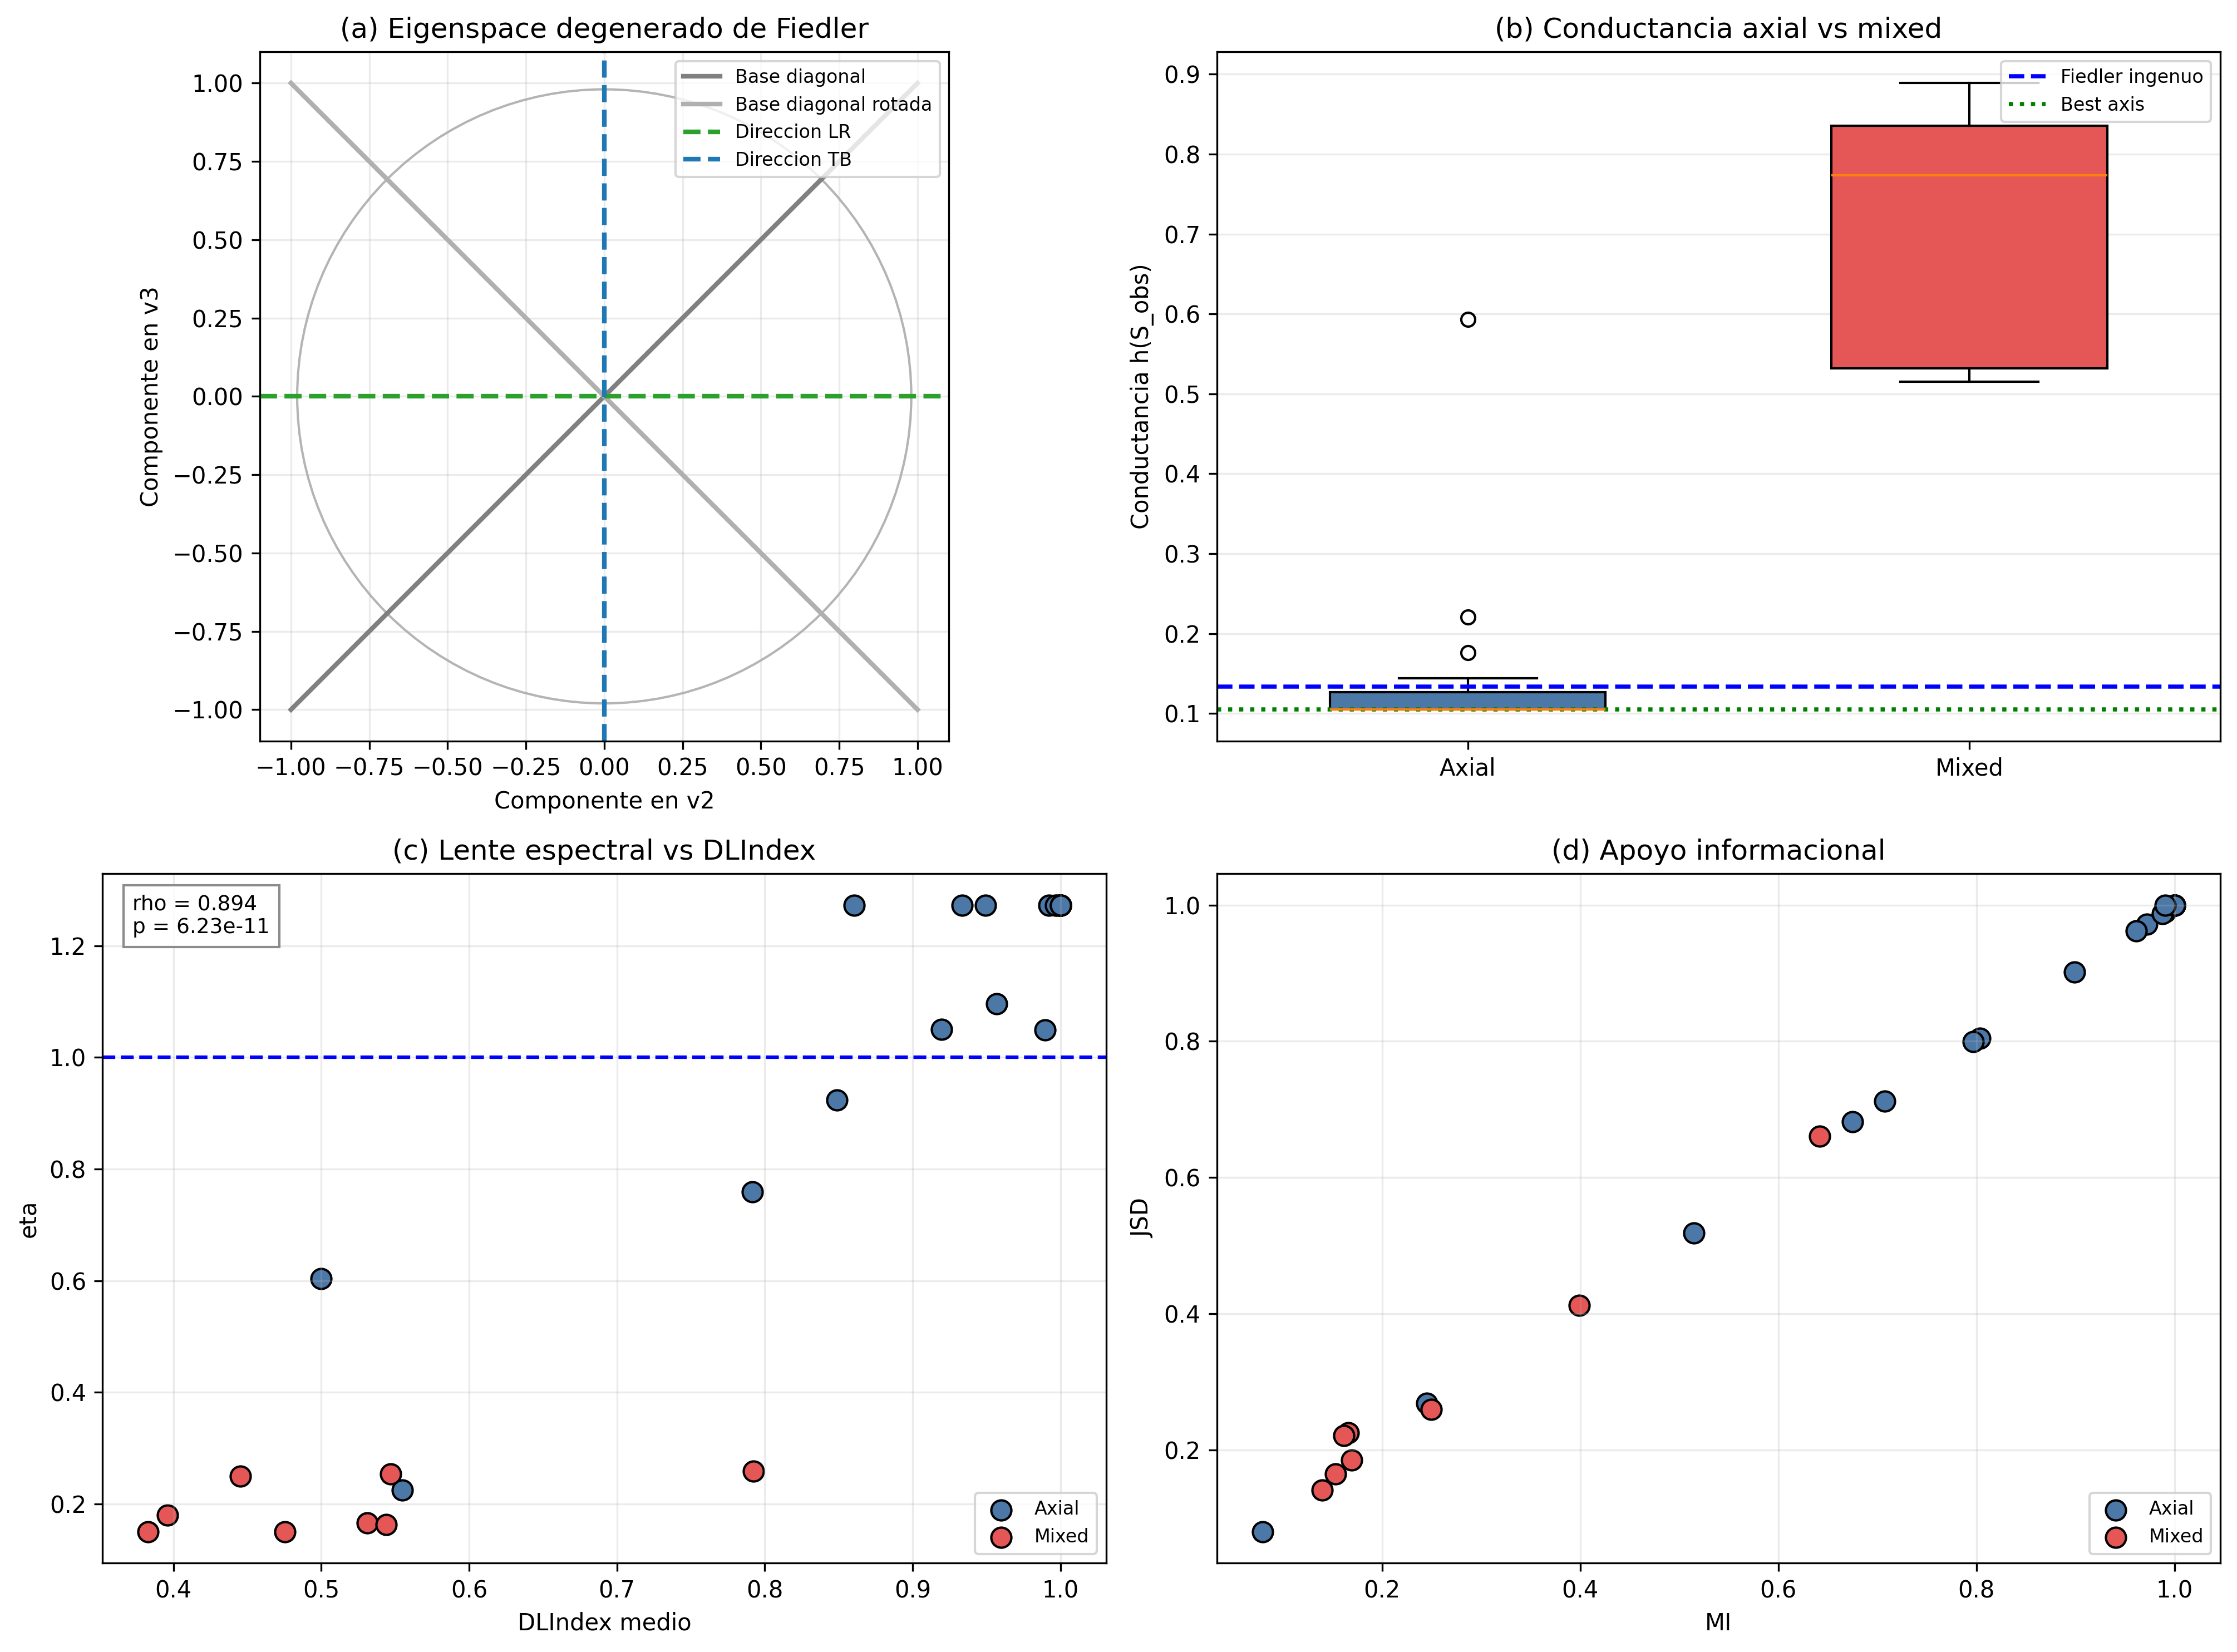
\includegraphics[width=\columnwidth]{andrade_summary.png}
\caption{Resumen del reanalisis: eigenspace degenerado, separacion axial vs mixed en conductancia, relacion entre $\eta$ y DLIndex, y apoyo informacional mediante MI/JSD.}
\label{fig:andrade}
\end{figure}

\subsection{Gate de novedad}

El reanalisis pasa un primer filtro descriptivo, pero no un filtro fuerte de novedad independiente. La correlacion de Spearman entre $\eta$ y $DLIndex$ es $\rho=0.894$ con $p=6.23\times10^{-11}$. Esto sugiere que la conductancia espectral no esta capturando una dimension completamente ortogonal a la medida original de Andrade-Lotero y Goldstone \cite{andrade2021}. Lo que agrega es, sobre todo, una lectura geometrica de por que ciertas convenciones axiales son privilegiadas en el caso cuadrado.

\section{Discusion critica}

El resultado positivo de este proyecto es real: en el tablero cuadrado, la degeneracion del eigenspace de Fiedler convive con una separacion empirica fuerte entre diadas axiales y mixtas. Cuando la organizacion humana adopta una biparticion espacial clara, esa organizacion suele caer cerca de las direcciones LR/TB que el propio entorno hace geometricamente privilegiadas.

Sin embargo, el proyecto no debe venderse como un paper cerrado todavia. Hay al menos tres limites de carga alta:
\begin{enumerate}
\item el baseline axis-aligned trivial empata numericamente al baseline espectral sensible a simetria en $P_8 \boxtimes P_8$;
\item $\eta$ y $DLIndex$ estan fuertemente acoplados, de modo que la novedad actual es interpretativa mas que dimensional;
\item el filtro de conductancia deja fuera precisamente muchas diadas ``ALL/NOTHING/RS'', asi que la explicacion es parcial incluso dentro del dataset original.
\end{enumerate}

Por eso, la mejor lectura del trabajo no es ``los humanos optimizan espectralmente'', sino algo mas sobrio: \textbf{la simetria del entorno induce una familia degenerada de direcciones espectralmente equivalentes, y varias diadas humanas seleccionan las direcciones axiales privilegiadas dentro de esa familia.} Esa observacion merece existir, pero pide una extension predictiva si se quiere convertir en una contribucion mas fuerte.

La extension natural es experimental y geometrica: romper la simetria del tablero. Si se pasa de un cuadrado a un rectangulo o a una version ligeramente perturbada, la prediccion es que la multiplicidad de $\lambda_2$ debe colapsar, la ambiguedad entre convenciones axiales debe reducirse y la distribucion de estrategias humanas deberia cambiar de forma sistematica. Esa es la ruta mas limpia para transformar este reanalisis en una pregunta publicable.

\section{Conclusion}

El proyecto, en su estado actual, sostiene una tesis acotada y defendible. La estructura espectral de $P_8 \boxtimes P_8$ ayuda a reinterpretar la coordinacion axial humana observada en SODCL, y las metricas de informacion y estabilidad refuerzan esa separacion. Pero el mismo analisis tambien impone sus propios limites: no explica todo el fenomeno, no destrona por si solo a los baselines cartesianos y no reemplaza la medida original del paper de 2021. Como resultado, este repositorio ya sirve como coursework fuerte y como paquete serio para discutir con Andrade una extension basada en ruptura de simetria. Todavia no sirve, por si solo, como evidencia suficiente de ``optimizacion espectral humana'' en sentido amplio.

\bibliographystyle{IEEEtran}
\begin{thebibliography}{12}

\bibitem{andrade2021}
E. Andrade-Lotero and R. L. Goldstone, ``Self-organized division of cognitive labor,'' \textit{PLOS ONE}, vol. 16, no. 7, p. e0254532, Jul. 2021.

\bibitem{chung1997}
F. R. K. Chung, \textit{Spectral Graph Theory}. Providence, RI: American Mathematical Society, 1997.

\bibitem{fiedler1973}
M. Fiedler, ``Algebraic connectivity of graphs,'' \textit{Czechoslovak Mathematical Journal}, vol. 23, no. 2, pp. 298--305, 1973.

\bibitem{mesbahi2010}
M. Mesbahi and M. Egerstedt, \textit{Graph Theoretic Methods in Multiagent Networks}. Princeton, NJ: Princeton University Press, 2010.

\bibitem{vonluxburg2007}
U. von Luxburg, ``A tutorial on spectral clustering,'' \textit{Statistics and Computing}, vol. 17, no. 4, pp. 395--416, Dec. 2007.

\bibitem{cheeger1970}
J. Cheeger, ``A lower bound for the smallest eigenvalue of the Laplacian,'' in \textit{Problems in Analysis}, Princeton, NJ: Princeton University Press, 1970, pp. 195--199.

\bibitem{mohar1991}
B. Mohar, ``The Laplacian spectrum of graphs,'' in \textit{Graph Theory, Combinatorics, and Applications}, vol. 2, Y. Alavi et al., Eds. New York: Wiley, 1991, pp. 871--898.

\bibitem{hammack2011}
R. Hammack, W. Imrich, and S. Klav\v{z}ar, \textit{Handbook of Product Graphs}, 2nd ed. Boca Raton, FL: CRC Press, 2011.

\bibitem{cover2006}
T. M. Cover and J. A. Thomas, \textit{Elements of Information Theory}, 2nd ed. Hoboken, NJ: Wiley-Interscience, 2006.

\bibitem{lin1991}
J. Lin, ``Divergence measures based on the Shannon entropy,'' \textit{IEEE Transactions on Information Theory}, vol. 37, no. 1, pp. 145--151, Jan. 1991.

\bibitem{newman2018}
M. Newman, \textit{Networks}, 2nd ed. Oxford: Oxford University Press, 2018.

\bibitem{goldstone2024}
R. L. Goldstone, E. Andrade-Lotero, R. D. Hawkins, and M. E. Roberts, ``The emergence of specialized roles within groups,'' \textit{Topics in Cognitive Science}, 2024.

\end{thebibliography}

\end{document}
